% =============================================================================
%  fig_system_architecture.tex
%  System architecture: synchronous generator → network → relay → adaptation
%  Compile standalone:  pdflatex fig_system_architecture.tex
% =============================================================================
\documentclass[tikz, border=6pt]{standalone}
\usepackage{tikz}
\usepackage{amsmath,amssymb}
\usetikzlibrary{shapes.geometric, shapes.misc, arrows.meta, positioning,
                fit, backgrounds, calc, decorations.pathreplacing}

% ---- colour palette (IEEE-compatible, greyscale-safe) -----------------------
\definecolor{genBlue}   {RGB}{31,  119, 180}
\definecolor{netGreen}  {RGB}{44,  160,  44}
\definecolor{relayRed}  {RGB}{214,  39,  40}
\definecolor{adaptPurp} {RGB}{148, 103, 189}
\definecolor{boxGray}   {RGB}{248, 248, 248}
\definecolor{arrowGray} {RGB}{100, 100, 100}

\tikzset{
  blk/.style = {rectangle, rounded corners=3pt, draw=#1, fill=boxGray,
                line width=0.9pt, text width=2.8cm, align=center,
                minimum height=1.1cm, font=\small},
  subblk/.style = {rectangle, rounded corners=2pt, draw=#1!70, fill=#1!10,
                   line width=0.7pt, text width=2.4cm, align=center,
                   minimum height=0.85cm, font=\footnotesize},
  arr/.style  = {-{Stealth[length=5pt]}, line width=0.9pt, color=arrowGray},
  garr/.style = {-{Stealth[length=5pt]}, line width=1.1pt, color=#1},
  lbl/.style  = {font=\scriptsize, align=center, color=gray!70!black},
  grpbox/.style = {rectangle, rounded corners=4pt, draw=#1!60, fill=#1!5,
                   line width=0.8pt, dashed},
}

\begin{document}
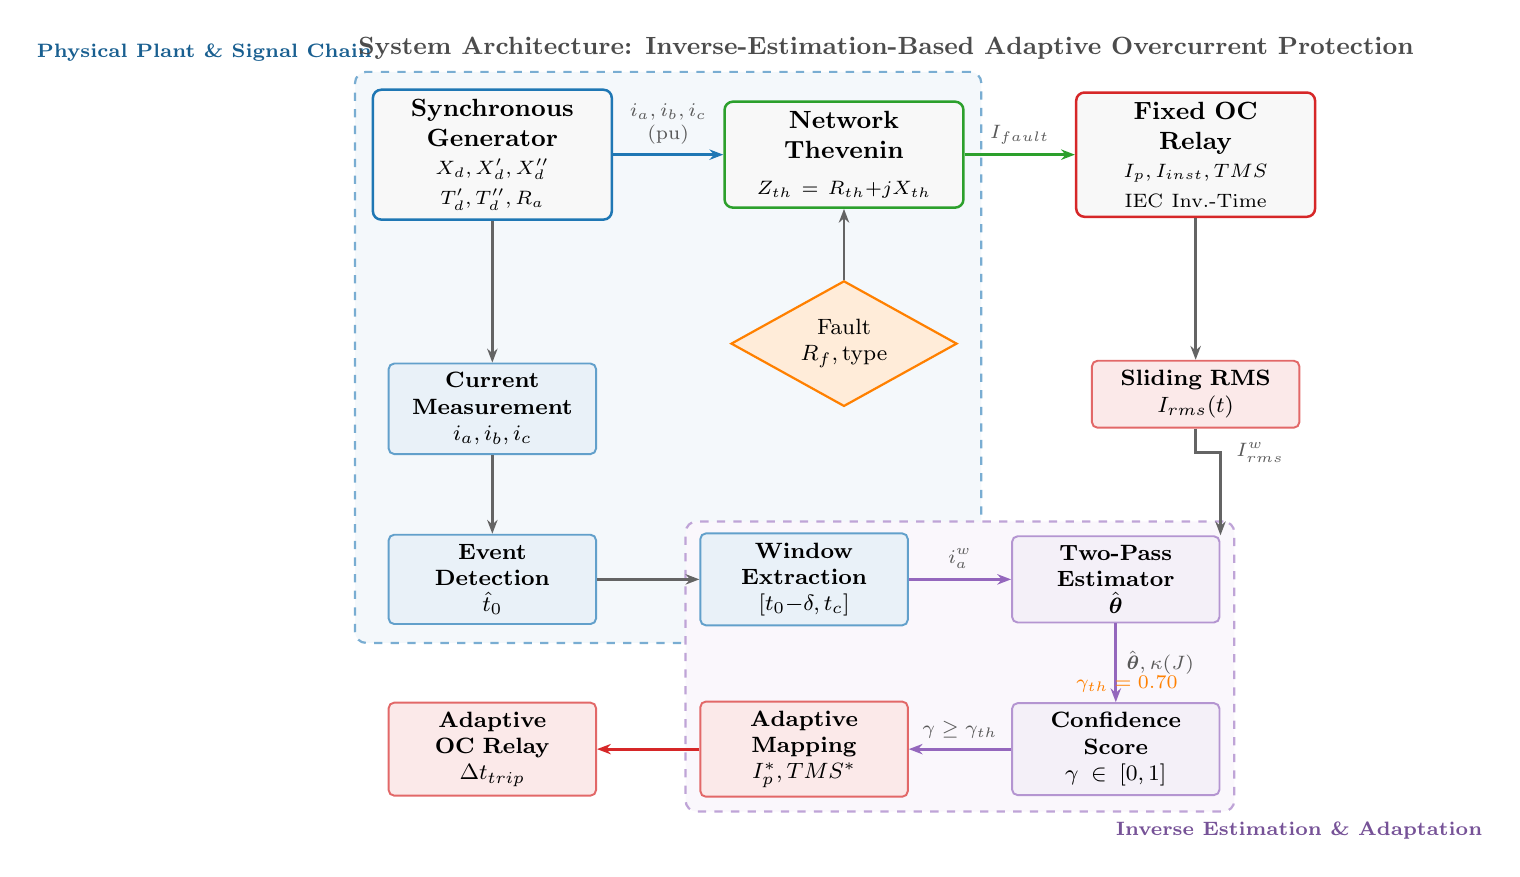
\begin{tikzpicture}[node distance=0.55cm and 1.2cm]

% ---- Row 1: Physical plant --------------------------------------------------
\node[blk=genBlue] (gen) {%
  \textbf{Synchronous}\\\textbf{Generator}\\[2pt]
  \scriptsize $X_d, X_d', X_d''$\\$T_d', T_d'', R_a$};

\node[blk=netGreen, right=1.4cm of gen] (net) {%
  \textbf{Network}\\\textbf{Thevenin}\\[2pt]
  \scriptsize $Z_{th}=R_{th}{+}jX_{th}$};

\node[blk=relayRed, right=1.4cm of net] (relay) {%
  \textbf{Fixed OC}\\\textbf{Relay}\\[2pt]
  \scriptsize $I_p, I_{inst}, TMS$\\IEC Inv.-Time};

% ---- Fault injection --------------------------------------------------------
\node[draw=orange, fill=orange!15, diamond, aspect=1.8, font=\footnotesize,
      below=0.9cm of net, align=center, line width=0.8pt] (fault)
      {Fault\\$R_f, \text{type}$};

% ---- Row 2: Measurement chain -----------------------------------------------
\node[subblk=genBlue, below=1.8cm of gen] (meas) {%
  \textbf{Current}\\\textbf{Measurement}\\$i_a, i_b, i_c$};

\node[subblk=relayRed, below=1.8cm of relay] (rms) {%
  \textbf{Sliding RMS}\\$I_{rms}(t)$};

% ---- Row 3: Estimation chain ------------------------------------------------
\node[subblk=genBlue, below=1.0cm of meas] (detect) {%
  \textbf{Event}\\\textbf{Detection}\\$\hat{t}_0$};

\node[subblk=genBlue, right=1.3cm of detect] (window) {%
  \textbf{Window}\\\textbf{Extraction}\\$[t_0{-}\delta, t_c]$};

\node[subblk=adaptPurp, right=1.3cm of window] (estim) {%
  \textbf{Two-Pass}\\\textbf{Estimator}\\$\hat{\boldsymbol{\theta}}$};

% ---- Row 4: Confidence + adaptation -----------------------------------------
\node[subblk=adaptPurp, below=1.0cm of estim] (conf) {%
  \textbf{Confidence}\\\textbf{Score}\\$\gamma \in [0,1]$};

\node[subblk=relayRed, left=1.3cm of conf] (map) {%
  \textbf{Adaptive}\\\textbf{Mapping}\\$I_p^*, TMS^*$};

\node[subblk=relayRed, left=1.3cm of map] (adaptrelay) {%
  \textbf{Adaptive}\\\textbf{OC Relay}\\$\Delta t_{trip}$};

% ---- Arrows: physical plant -------------------------------------------------
\draw[garr=genBlue]  (gen) -- node[above,lbl]{$i_a,i_b,i_c$\\(pu)} (net);
\draw[garr=netGreen] (net) -- node[above,lbl]{$I_{fault}$} (relay);
\draw[arr]           (fault) -- (net);

% ---- Arrows: measurement chain ----------------------------------------------
\draw[arr] (gen.south) -- ++(0,-0.4) -| (meas.north);
\draw[arr] (relay.south) -- ++(0,-0.4) -| (rms.north);

% ---- Arrows: estimation chain -----------------------------------------------
\draw[arr] (meas) -- (detect);
\draw[arr] (detect) -- (window);
\draw[garr=adaptPurp] (window) -- node[above,lbl]{$i_a^w$} (estim);
\draw[arr] (rms.south) -- ++(0,-0.3) -| node[right,lbl,xshift=2pt]{$I_{rms}^w$} (estim.north east);

% ---- Arrows: adaptation chain -----------------------------------------------
\draw[garr=adaptPurp] (estim) -- node[right,lbl]{$\hat{\boldsymbol{\theta}},\kappa(J)$} (conf);
\draw[garr=adaptPurp] (conf) -- node[above,lbl]{$\gamma \geq \gamma_{th}$} (map);
\draw[garr=relayRed]  (map) -- (adaptrelay);

% ---- Gate annotation --------------------------------------------------------
\node[font=\scriptsize, text=orange, above=0pt of conf, xshift=4pt]
      {$\gamma_{th}=0.70$};

% ---- Group boxes (backgrounds) ----------------------------------------------
\begin{scope}[on background layer]
  \node[grpbox=genBlue, fit=(gen)(net)(meas)(detect)(window), inner sep=6pt,
        label={[font=\scriptsize\bfseries, text=genBlue!80!black]above left:Physical Plant \& Signal Chain}] {};
  \node[grpbox=adaptPurp, fit=(estim)(conf)(map), inner sep=5pt,
        label={[font=\scriptsize\bfseries, text=adaptPurp!80!black]below right:Inverse Estimation \& Adaptation}] {};
\end{scope}

% ---- Title ------------------------------------------------------------------
\node[font=\small\bfseries, above=0.25cm of gen, xshift=5cm, text=black!70]
     {System Architecture: Inverse-Estimation-Based Adaptive Overcurrent Protection};

\end{tikzpicture}
\end{document}
